\documentclass[14pt, a4paper]{extarticle}

\usepackage[utf8]{inputenc}
\usepackage[T1]{fontenc}
\usepackage{amsmath}
\usepackage{amssymb}
\usepackage{graphicx}
\usepackage[left=2.00cm, right=2.00cm, top=2.00cm, bottom=2.00cm]{geometry}
\usepackage[russian]{babel}

\usepackage{setspace}
\usepackage{fancyhdr}

\graphicspath{{img/}}

\RequirePackage{caption}
\captionsetup[figure]{justification=centering,name=Рисунок,labelsep=endash}

\usepackage{indentfirst}

\usepackage{float}

\usepackage{titlesec}
\titleformat{\section}{\normalfont\bfseries}{\thesection~}{0em}{}

\begin{document}
	\onehalfspacing
	\begin{titlepage}
	\begin{center}
		\begin{small}
			\textbf{Министерство науки и высшего образования Российской Федерации}

			ФЕДЕРАЛЬНОЕ ГОСУДАРСТВЕННОЕ АВТОНОМНОЕ ОБРАЗОВАТЕЛЬНОЕ УЧРЕЖДЕНИЕ ВЫСШЕГО ОБРАЗОВАНИЯ
			
			\textbf{<<НАЦИОНАЛЬНЫЙ ИССЛЕДОВАТЕЛЬСКИЙ УНИВЕРСИТЕТ ИТМО>>}
		\end{small}
		
		\vspace{8em}
		
		Отчет по лабораторной работе №4
		
		РОБАСТНОЕ УПРАВЛЕНИЕ ЛИНЕЙНЫМ МНОГОМЕРНЫМ ОБЪЕКТОМ ПО СОСТОЯНИЮ
		
		По дисциплине <<Адаптивное и робастное управление>>
	\end{center}
	
	\vspace{8em}
	
	\begin{flushright}
		Выполнил:\\
		студент группы R42331c\\
		Манахов~С.П.
		
		\vspace{1em}
		
		Преподаватель:\\
		Парамонов~А.В.
	\end{flushright}

	\vfill
	
	\begin{center}
		\small
		Санкт-Петербург\\
		2022 г.\\
	\end{center}
\end{titlepage}
	\setcounter{page}{2}
	
	\section*{Задание}
	
	Дан объект:
	$$\begin{matrix}
		\dot{x} = Ax + bu, x(0),\\
		y = Cx,
	\end{matrix}$$
	где $x\in R^n$ -- вектор состояния, $u$ -- управление, $y \in R$ -- регулируемая переменная,
	$$A=\left[\begin{matrix}
		0 & 1 & 0 & \cdots & 0 \\
		0 & 0 & 1 & \cdots & 0 \\
		\vdots & \vdots & \vdots & \ddots & \vdots \\
		0 & 0 & 0 & \cdots & 1 \\
		-a_0 & -a_1 & -a_2 & \cdots & -a_{n-1} \\
	\end{matrix}\right], b = \left[\begin{matrix}
		0 \\ 0 \\ \vdots \\ 0 \\ b_0 \\
	\end{matrix}\right], C = \left[\begin{matrix}
		1 & 0 & \cdots & 0 & 0
	\end{matrix}\right],$$
	$a_i, i=\overline{0,n-1}$ -- неизвестные параметры, $b_0$ -- известный коэффициент.
	
	Задача управления заключается в компенсации параметрической неопределенности объекта и обеспечении следующего целевого равенства:
	$$\lim\limits_{t\to\infty}\left|\left|x_M(t)-x(t)\right|\right|=\lim\limits_{t\to\infty}\left|\left|e(t)\right|\right|=0,$$
	где $e=x_M-x$ -- вектор ошибки управления, $x_M\in R^n$ --вектор, генерируемый эталонной моделью:
	$$\begin{matrix}
		\dot{x}_M = A_Mx_M + b_Mg,\\
		y_M = C_Mx_M
	\end{matrix}$$
	с задающим воздействием $g(t)$ и матрицами:
	$$A_M=\left[\begin{matrix}
		0 & 1 & 0 & \cdots & 0 \\
		0 & 0 & 1 & \cdots & 0 \\
		\vdots & \vdots & \vdots & \ddots & \vdots \\
		0 & 0 & 0 & \cdots & 1 \\
		-a_{M0} & -a_{M1} & -a_{M2} & \cdots & -a_{Mn-1} \\
	\end{matrix}\right], b_M = \left[\begin{matrix}
		0 \\ 0 \\ \vdots \\ 0 \\ a_{M0} \\
	\end{matrix}\right],$$
	$$C_M = \left[\begin{matrix}
		1 & 0 & \cdots & 0 & 0
	\end{matrix}\right]$$

	Параметры эталонной модели $a_{Mi},i=\overline{1,n-1}$ строятся на основе метода стандартных характеристических полиномов для обеспечения желаемого качества воспроизведения задающего воздействия $g(t)$. Другими словами, модель определяет желаемое качество замкнутой системы после завершения процессов настройки адаптивного управления.

	\begin{enumerate}
		\item На основе заданных в таблице значений времени переходного процесса $t_\text{п}$ и максимального перерегулирования $\bar{\sigma}$ сформировать эталонную модель. Построить график переходной функции модели, на котором показать время переходного процесса $t_\text{п}$ и перерегулирование $\bar{\sigma}$;
		\item На основе предположения, что параметры объекта известны, построить и промоделировать систему управления с регулятором. Провести три эксперимента, в которых:
		\subitem -- использовать расчетные значения параметров объекта, заложенные в $\theta_1$ и $\theta_2$;
		\subitem -- незначительно отклонить параметры объекта так, чтобы система не потеряла устойчивость;
		\subitem -- отклонить параметры объекта так, чтобы система потеряла устойчивость.
		
		По результатам каждого эксперимента построить траектории $x(t)$ и $x_M(t)$ на одном графике и $e(t)$ -- на другом;
		\item Провести моделирование адаптивной системы управления с регулятором и алгоритмом адаптации. В ходе моделирования проиллюстрировать свойства 1-4 алгоритма управления. Для этого необходимо:
		\subitem -- повторить три эксперимента п.п.~2 для фиксированного значения $\gamma$;
		\subitem -- используя расчетные значения параметров объекта, провести эксперимент с тремя различными значениями $\gamma$;
		\subitem -- провести один из предыдущих экспериментов данного пункта при $g(t)=1$.
		
		По результатам каждого эксперимента построить траектории $x(t)$ и $x_M(t)$ на одном графике, $e(t)$ -- на втором, $\tilde{\theta}=\theta-\hat{\theta}$ -- на третьем;
		\item Сделать выводы по каждому пункту работы.
 	\end{enumerate}
	\begin{table}[H]
		\centering
		\begin{tabular}{|l|l|p{0.1\textwidth}|p{0.13\textwidth}|p{0.2\textwidth}|p{0.15\textwidth}|}
			\hline
			Вариант & Матрица $A$ & Коэф передачи $b_0$ & Время переходного процесса, $t_n$ & Максимального перерегулирование $\bar{\sigma}$, \% & Сигнал задания $g(t)$\\\hline
			18 & 
			$\left[
			\begin{matrix}
				0 & 1 \\
				-10 & 6 
			\end{matrix}
			\right]$
			& 9 & 0,15 & 15 & $0,8sin2t+cos0,8t+2$ \\\hline
		\end{tabular}
	\end{table}
	
	\newpage
	
	\section*{Описание работы}
	
	\begin{enumerate}
		\item Сформируем эталонную модель на основе заданных в таблице значений времени переходного процесса $t_\text{п}$ и максимального перерегулирования $\bar{\sigma}$. В качестве стандартного характеристического полинома будем использовать полином Баттерворта. 
		
		На рисунке \ref{fig:1-xm} представлен график переходной функции эталонной модели.
		
		\begin{figure}[H]
			\centering
			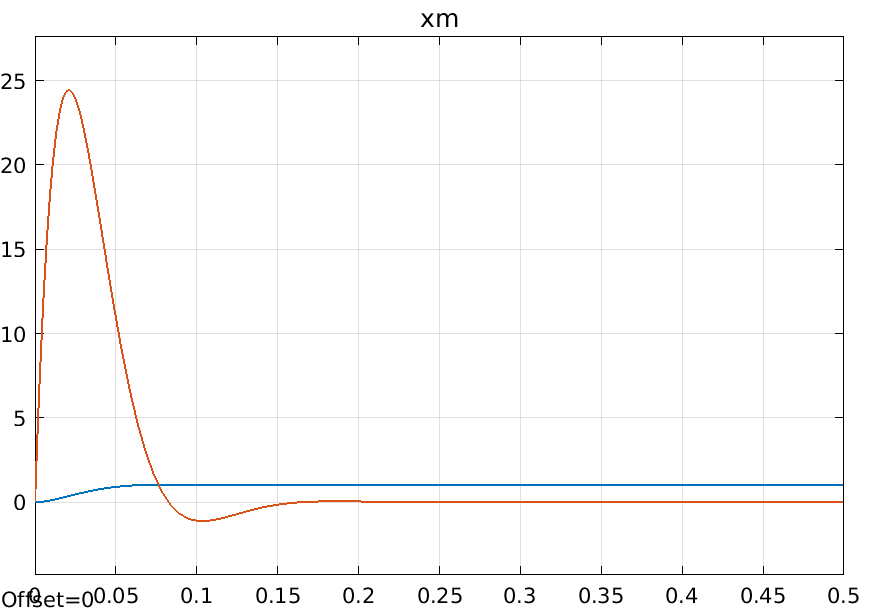
\includegraphics[width=0.59\textwidth]{1-xm}
			\caption{Переходная функция эталонной модели}
			\label{fig:1-xm}
		\end{figure}
		
		\item На основе предположения, что параметры объекта известны, промоделируем систему управления с регулятором:
		$$u=\theta^Tx+\frac{1}{\kappa}g$$
		где $\theta^T=\left[\begin{matrix}
			\theta_1, & \theta_2
		\end{matrix}\right]$ -- вектор неизвестных параметров, определяемый параметрическими рассогласованиями между матрицами $A$ и $A_M$,
		$$\theta_1=\frac{-a_{M0}+a_0}{b_0}, \theta_2=\frac{-a_{M1}+a_1}{b_0}, \kappa=\frac{b_0}{a_{M0}}$$
		
		Полученная система представлена на рисунках \ref{fig:2-system}-\ref{fig:2-properties}.
		
		\begin{figure}[H]
			\centering
			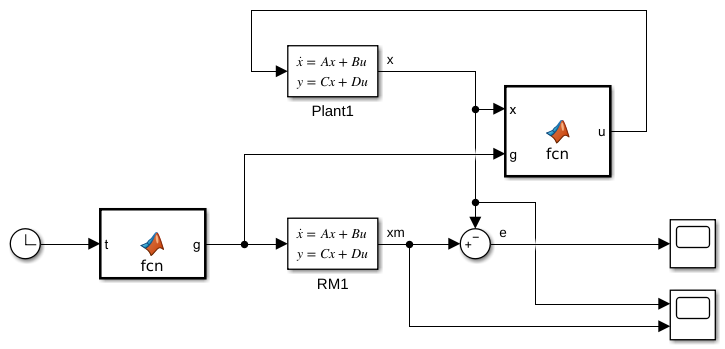
\includegraphics[width=0.59\textwidth]{2-system}
			\caption{Система управления при известных параметрах объекта}
			\label{fig:2-system}
		\end{figure}
		
		\begin{figure}[H]
			\centering
			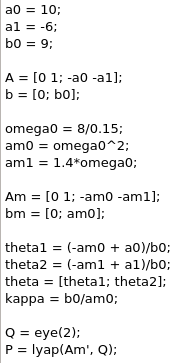
\includegraphics{2-properties}
			\caption{Параметры системы}
			\label{fig:2-properties}
		\end{figure}
		
		Полученные графики представлены на рисунках \ref{fig:2-1-x}, \ref{fig:2-1-e}.
		
		\begin{figure}[H]
			\centering
			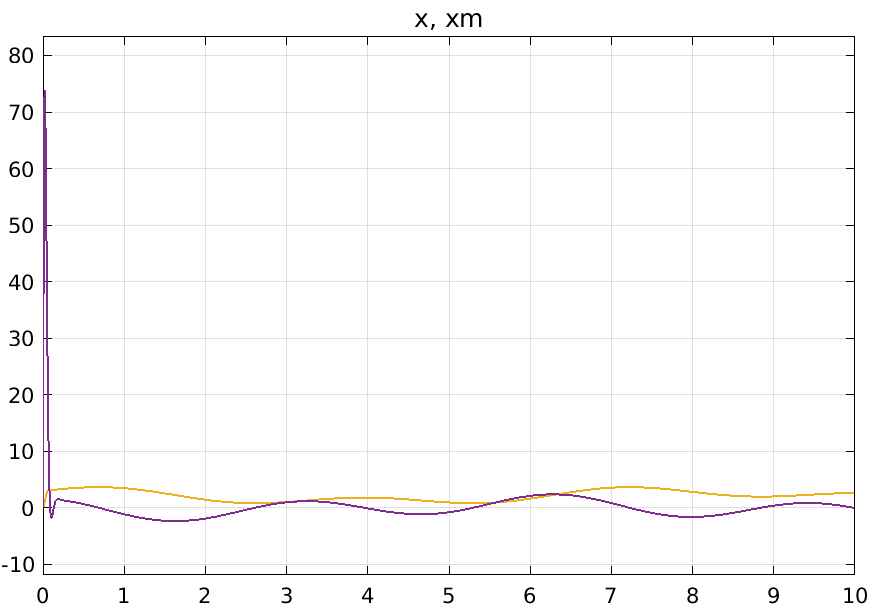
\includegraphics[width=0.59\textwidth]{2-1-x}
			\caption{Вектора состояния модели $x$ и эталонной модели $x_M$ }
			\label{fig:2-1-x}
		\end{figure}
		
		\begin{figure}[H]
			\centering
			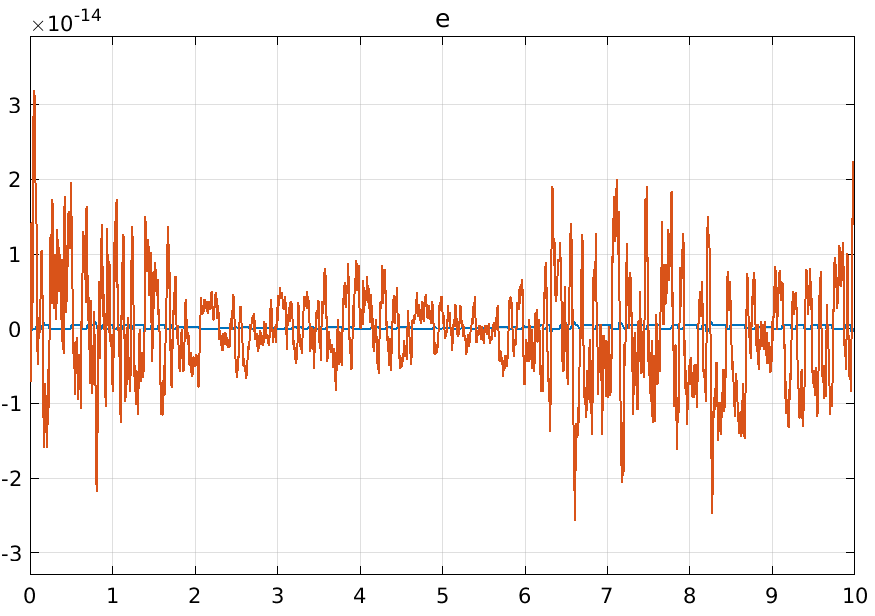
\includegraphics[width=0.59\textwidth]{2-1-e}
			\caption{Вектор ошибки управления $e$}
			\label{fig:2-1-e}
		\end{figure}
		
		Теперь отклоним параметры объекта следующим образом:
		$$A=\left[
		\begin{matrix}
			0 & 1 \\
			-a_0+50 & -a_1+50 
		\end{matrix}
		\right]$$
		
		При этом система не потеряла устойчивость. Полученные графики представлены на рисунках \ref{fig:2-2-x}, \ref{fig:2-2-e}.
		
		\begin{figure}[H]
			\centering
			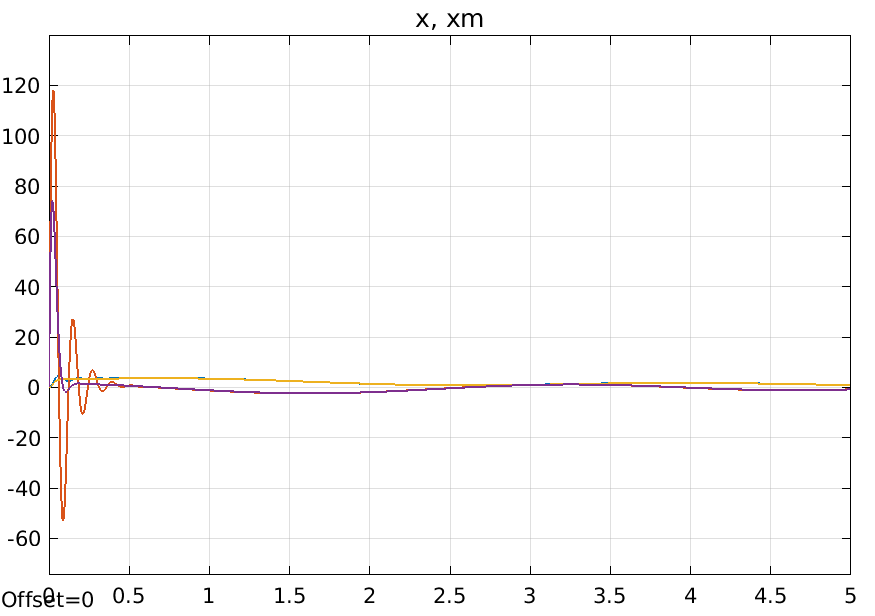
\includegraphics[width=0.59\textwidth]{2-2-x}
			\caption{Вектора состояния модели $x$ и эталонной модели $x_M$ при незначительном отклонении параметров объекта}
			\label{fig:2-2-x}
		\end{figure}
		
		\begin{figure}[H]
			\centering
			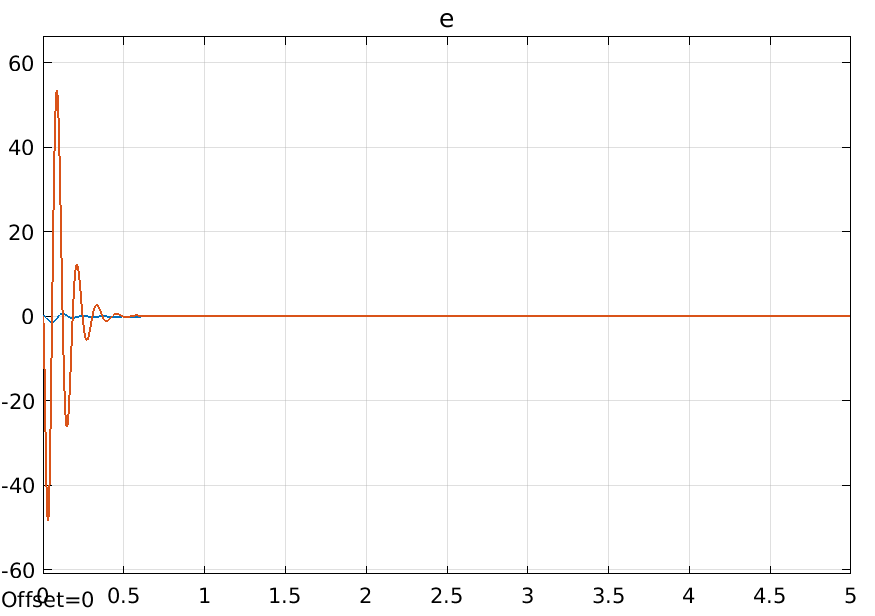
\includegraphics[width=0.59\textwidth]{2-2-e}
			\caption{Вектор ошибки управления $e$ при незначительном отклонении параметров объекта}
			\label{fig:2-2-e}
		\end{figure}
		
		Теперь отклоним параметры объекта следующим образом:
		$$A=\left[
		\begin{matrix}
			0 & 1 \\
			-a_0+100 & -a_1+100 
		\end{matrix}
		\right]$$
		
		При этом система потеряла устойчивость. Полученные графики представлены на рисунках \ref{fig:2-2-x}, \ref{fig:2-2-e}.
		
		\begin{figure}[H]
			\centering
			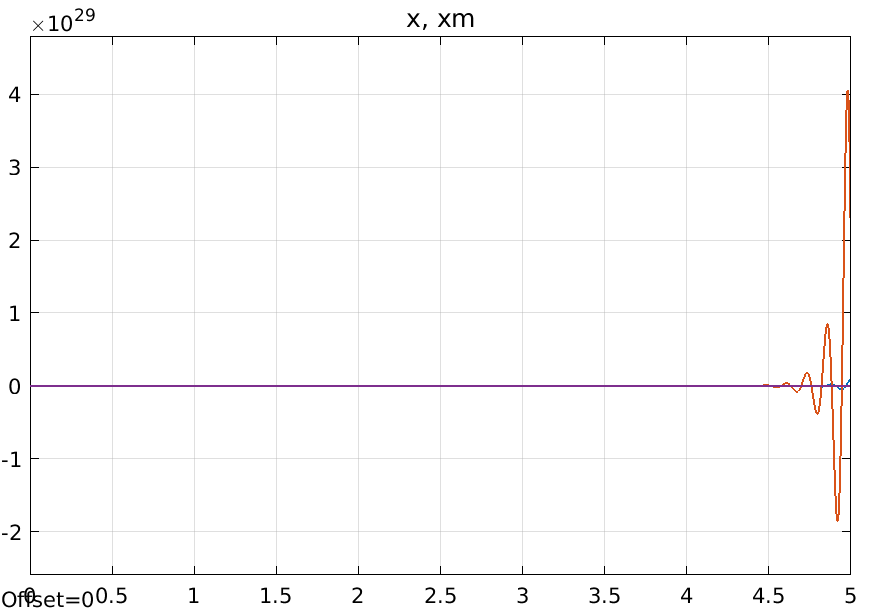
\includegraphics[width=0.59\textwidth]{2-3-x}
			\caption{Вектора состояния модели $x$ и эталонной модели $x_M$ при значительном отклонении параметров объекта}
			\label{fig:2-3-x}
		\end{figure}
		
		\begin{figure}[H]
			\centering
			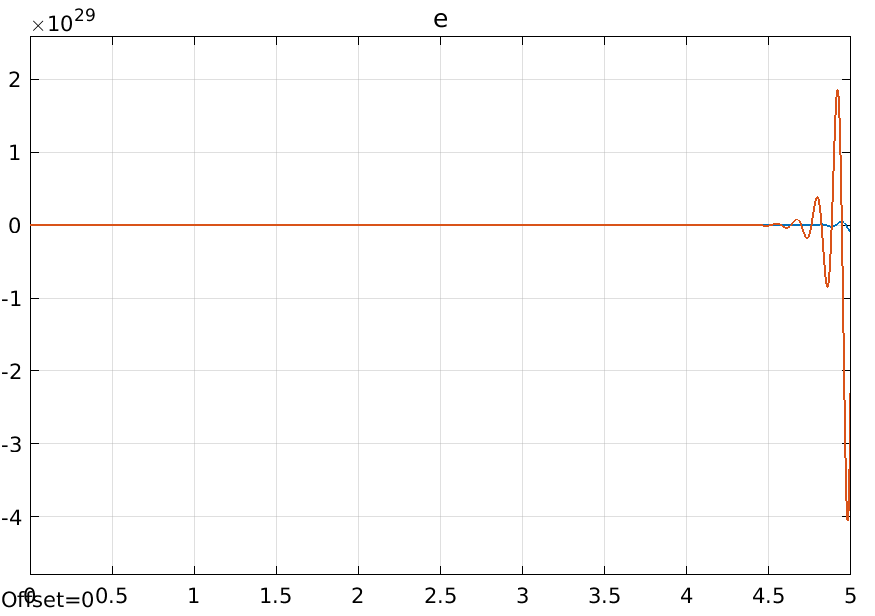
\includegraphics[width=0.59\textwidth]{2-3-e}
			\caption{Вектор ошибки управления $e$ при значительном отклонении параметров объекта}
			\label{fig:2-3-e}
		\end{figure}
		
		\item Теперь проведем моделирование адаптивной системы управления со следующими регулятором и алгоритмом адаптации:
		$$\begin{matrix}
			u=\hat{\theta}^Tx+\frac{1}{\kappa}g, & \dot{\hat{\theta}}=\gamma x b^TPe, & \hat{\theta}(0)=0
		\end{matrix}$$
		
		Полученная система представлена на рисунке \ref{fig:3-system}.
		
		\begin{figure}[H]
			\centering
			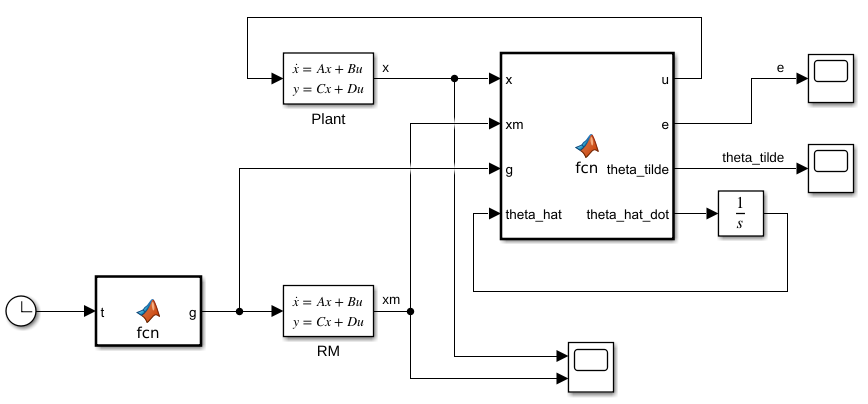
\includegraphics[width=0.59\textwidth]{3-system}
			\caption{Адаптивная система управления}
			\label{fig:3-system}
		\end{figure}
		
		Повторим три эксперимента п.п.~2 при $\gamma=100$. Полученные графики без отклонения параметров объекта представлены на рисунках \ref{fig:3-1-1-x}-\ref{fig:3-1-1-theta}. 
		
		\begin{figure}[H]
			\centering
			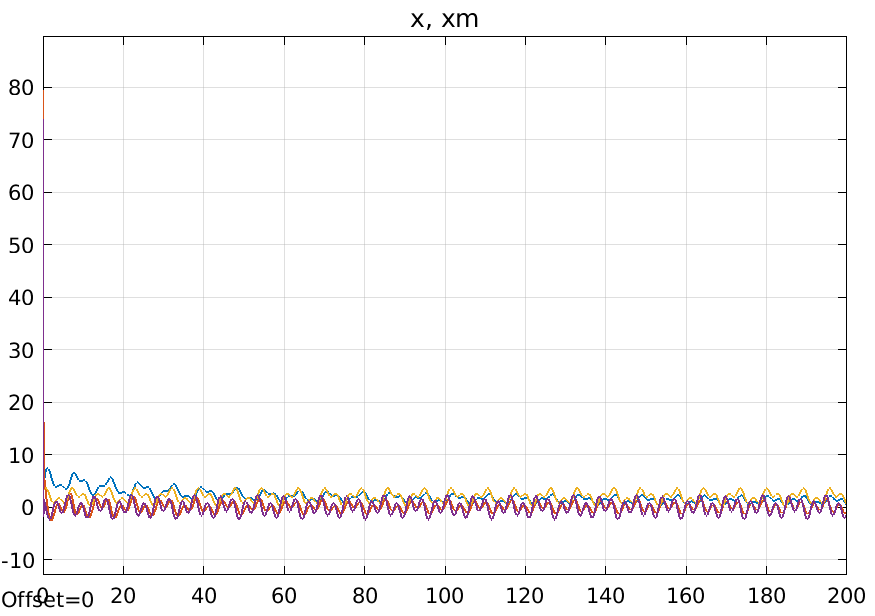
\includegraphics[width=0.59\textwidth]{3-1-1-x}
			\caption{Вектора состояния модели $x$ и эталонной модели $x_M$}
			\label{fig:3-1-1-x}
		\end{figure}
		
		\begin{figure}[H]
			\centering
			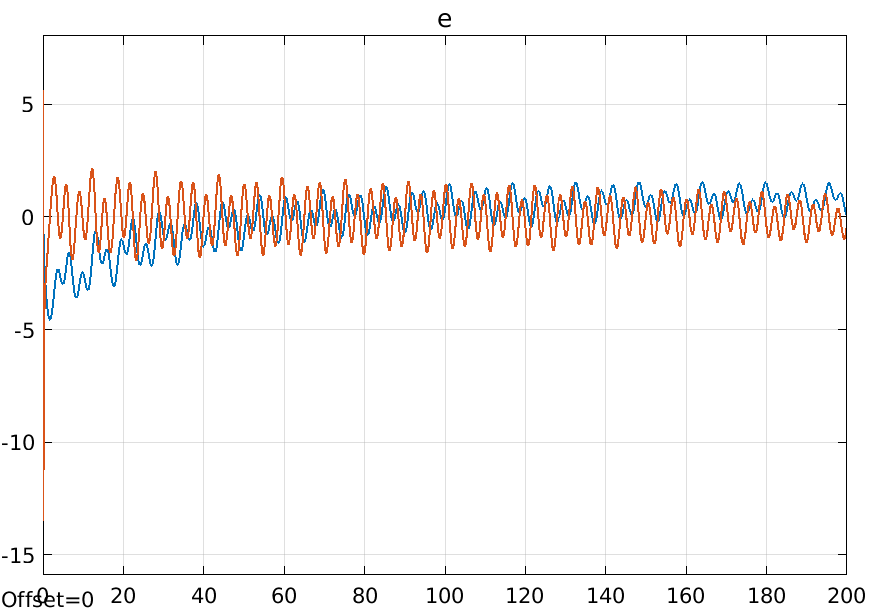
\includegraphics[width=0.59\textwidth]{3-1-1-e}
			\caption{Вектор ошибки управления $e$}
			\label{fig:3-1-1-e}
		\end{figure}
		
		\begin{figure}[H]
			\centering
			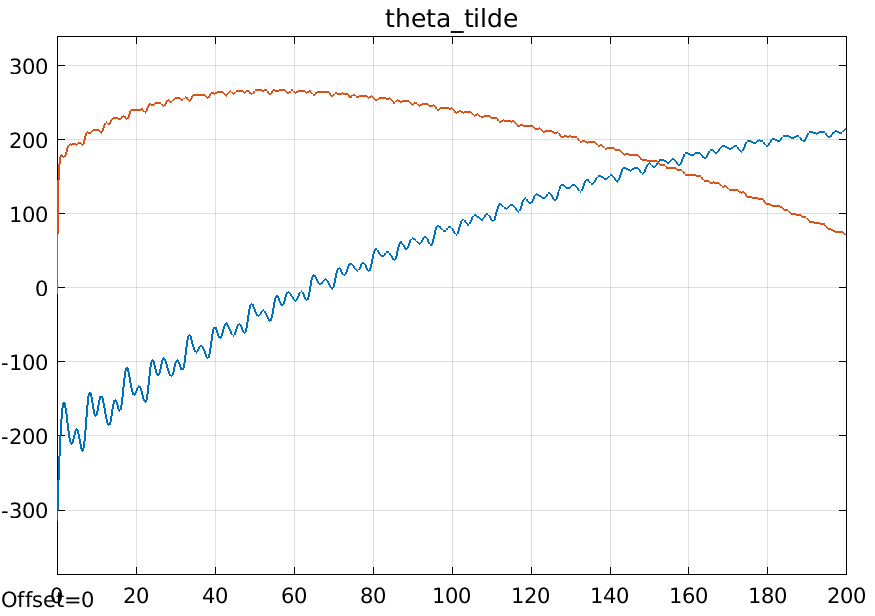
\includegraphics[width=0.59\textwidth]{3-1-1-theta}
			\caption{Вектор параметрических ошибок $\tilde{\theta}$}
			\label{fig:3-1-1-theta}
		\end{figure}
		
		Теперь отклоним параметры объекта следующим образом:
		$$A=\left[
		\begin{matrix}
			0 & 1 \\
			-a_0+50 & -a_1+50 
		\end{matrix}
		\right]$$
		
		Полученные графики представлены на рисунках \ref{fig:3-1-2-x}-\ref{fig:3-1-2-theta}. 
		
		\begin{figure}[H]
			\centering
			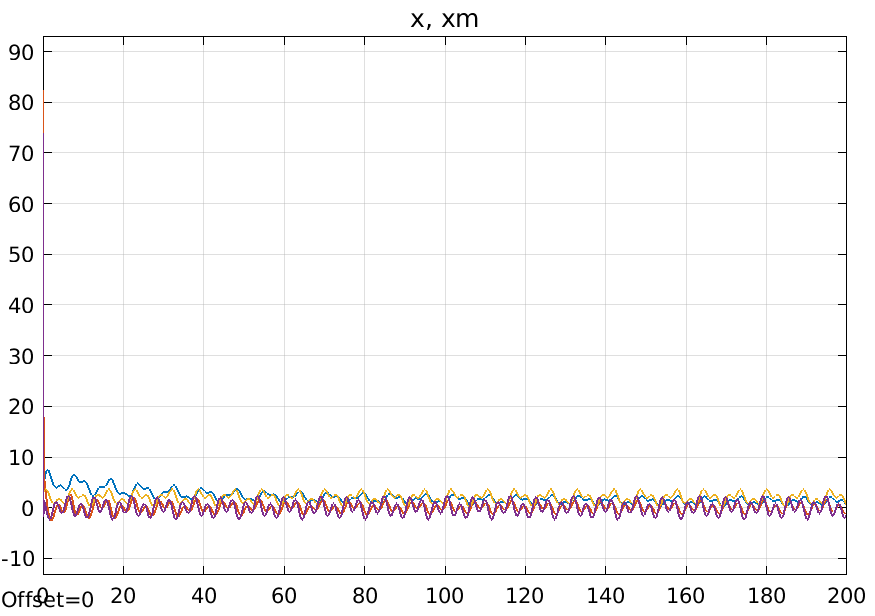
\includegraphics[width=0.59\textwidth]{3-1-2-x}
			\caption{Вектора состояния модели $x$ и эталонной модели $x_M$ при незначительном отклонении параметров объекта}
			\label{fig:3-1-2-x}
		\end{figure}
		
		\begin{figure}[H]
			\centering
			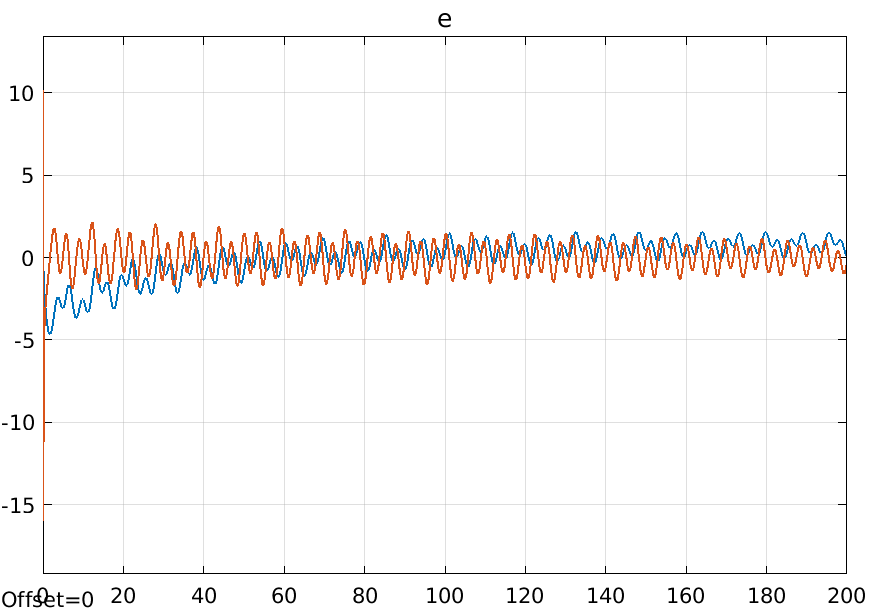
\includegraphics[width=0.59\textwidth]{3-1-2-e}
			\caption{Вектор ошибки управления $e$ при незначительном отклонении параметров объекта}
			\label{fig:3-1-2-e}
		\end{figure}
		
		\begin{figure}[H]
			\centering
			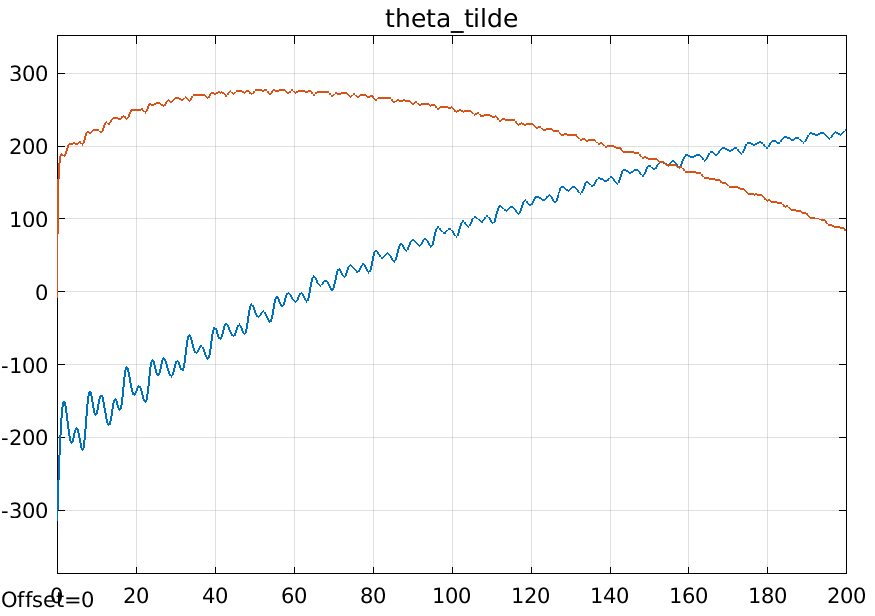
\includegraphics[width=0.59\textwidth]{3-1-2-theta}
			\caption{Вектор параметрических ошибок $\tilde{\theta}$ при незначительном отклонении параметров объекта}
			\label{fig:3-1-2-theta}
		\end{figure}
		
		Теперь отклоним параметры объекта следующим образом:
		$$A=\left[
		\begin{matrix}
			0 & 1 \\
			-a_0+100 & -a_1+100 
		\end{matrix}
		\right]$$
		
		Полученные графики представлены на рисунках \ref{fig:3-1-3-x}-\ref{fig:3-1-3-theta}. 
		
		\begin{figure}[H]
			\centering
			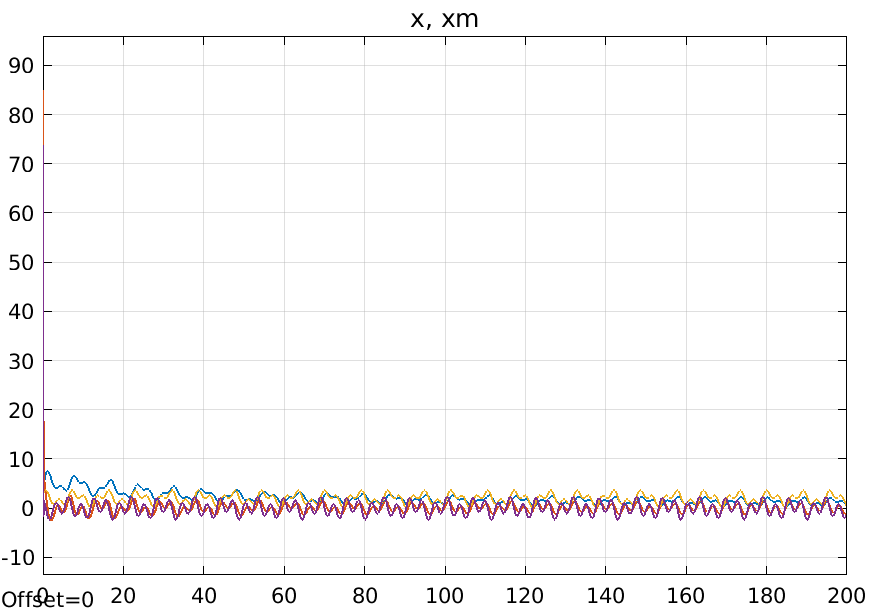
\includegraphics[width=0.59\textwidth]{3-1-3-x}
			\caption{Вектора состояния модели $x$ и эталонной модели $x_M$ при значительном отклонении параметров объекта}
			\label{fig:3-1-3-x}
		\end{figure}
		
		\begin{figure}[H]
			\centering
			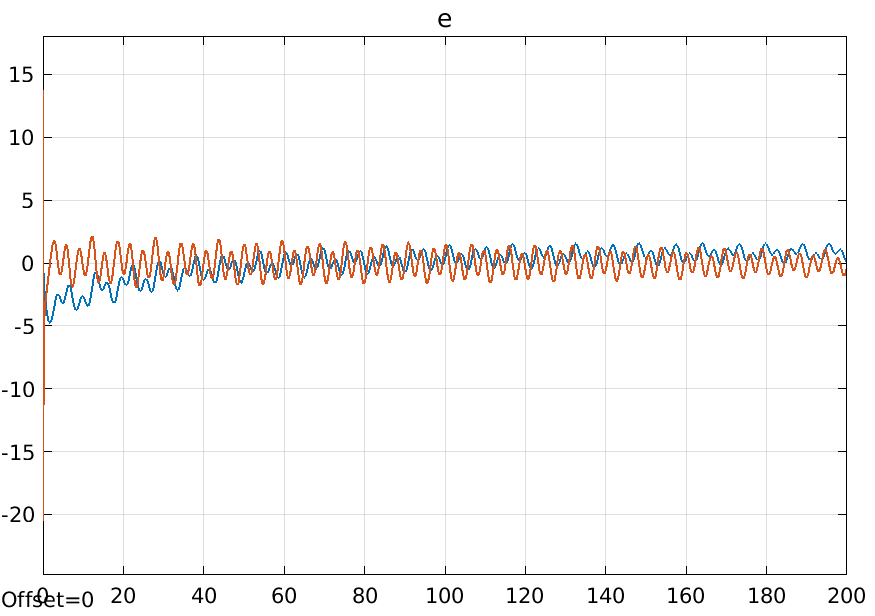
\includegraphics[width=0.59\textwidth]{3-1-3-e}
			\caption{Вектор ошибки управления $e$ при значительном отклонении параметров объекта}
			\label{fig:3-1-3-e}
		\end{figure}
		
		\begin{figure}[H]
			\centering
			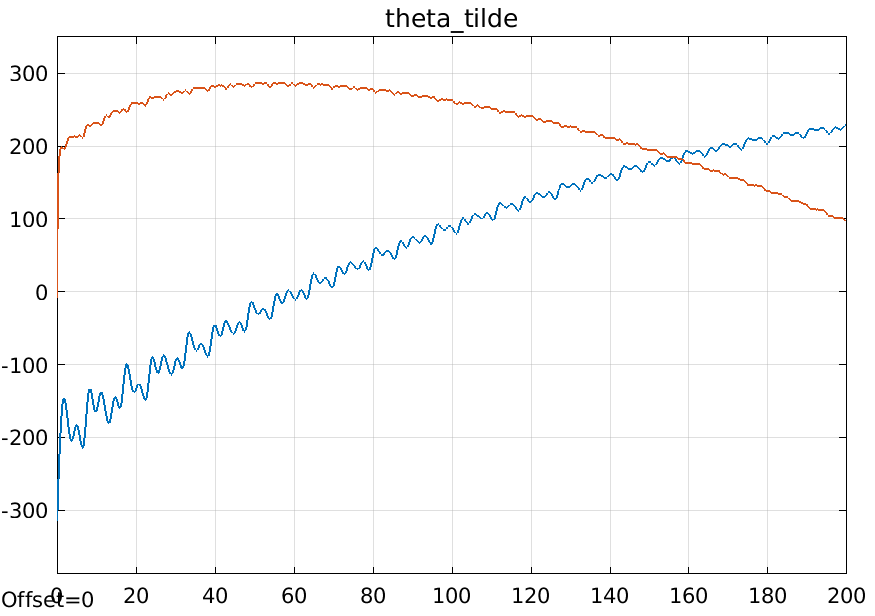
\includegraphics[width=0.59\textwidth]{3-1-3-theta}
			\caption{Вектор параметрических ошибок $\tilde{\theta}$ при значительном отклонении параметров объекта}
			\label{fig:3-1-3-theta}
		\end{figure}
		
		Теперь выберем $\gamma=1000$. Полученные графики представлены на рисунках \ref{fig:3-2-1-x}-\ref{fig:3-2-1-theta}.
		
		\begin{figure}[H]
			\centering
			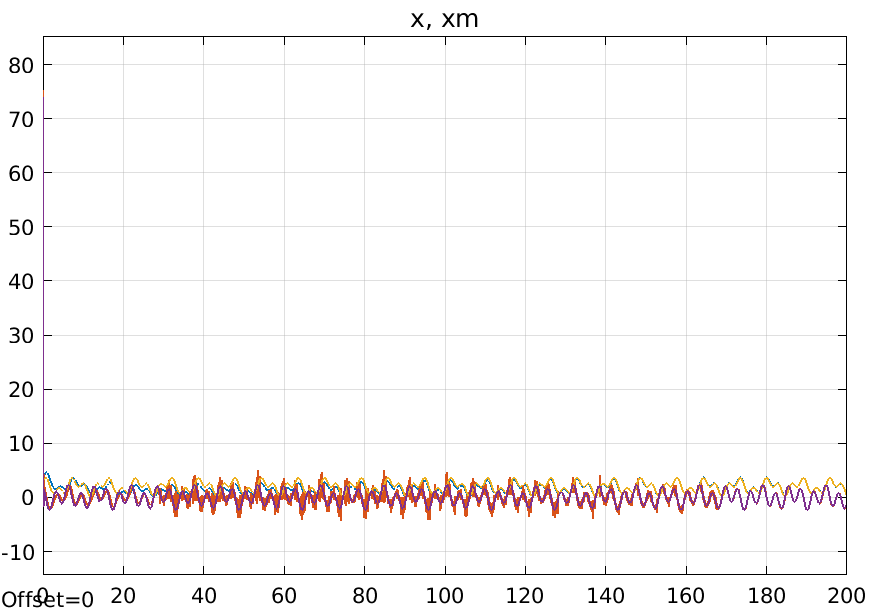
\includegraphics[width=0.59\textwidth]{3-2-1-x}
			\caption{Вектора состояния модели $x$ и эталонной модели $x_M$ при $\gamma=1000$}
			\label{fig:3-2-1-x}
		\end{figure}
		
		\begin{figure}[H]
			\centering
			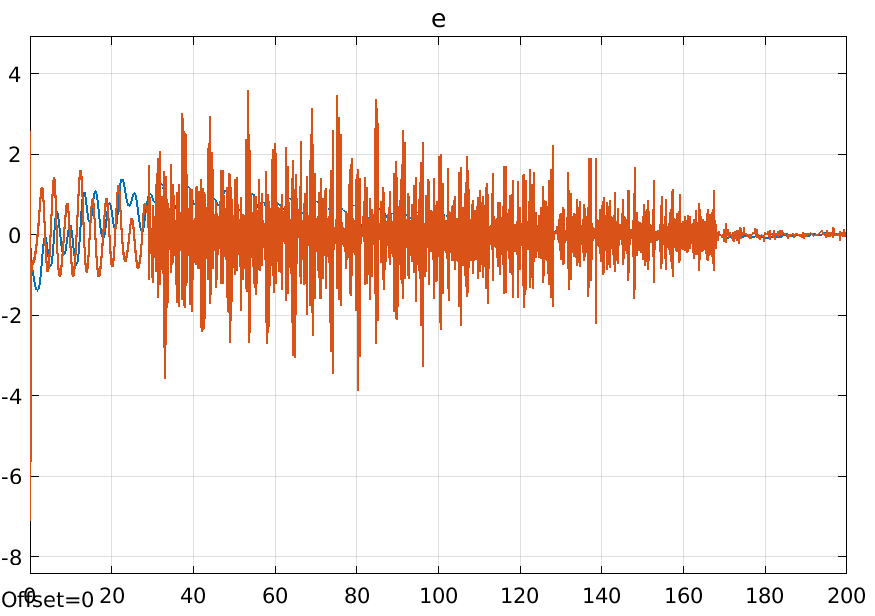
\includegraphics[width=0.59\textwidth]{3-2-1-e}
			\caption{Вектор ошибки управления $e$ при $\gamma=1000$}
			\label{fig:3-2-1-e}
		\end{figure}
		
		\begin{figure}[H]
			\centering
			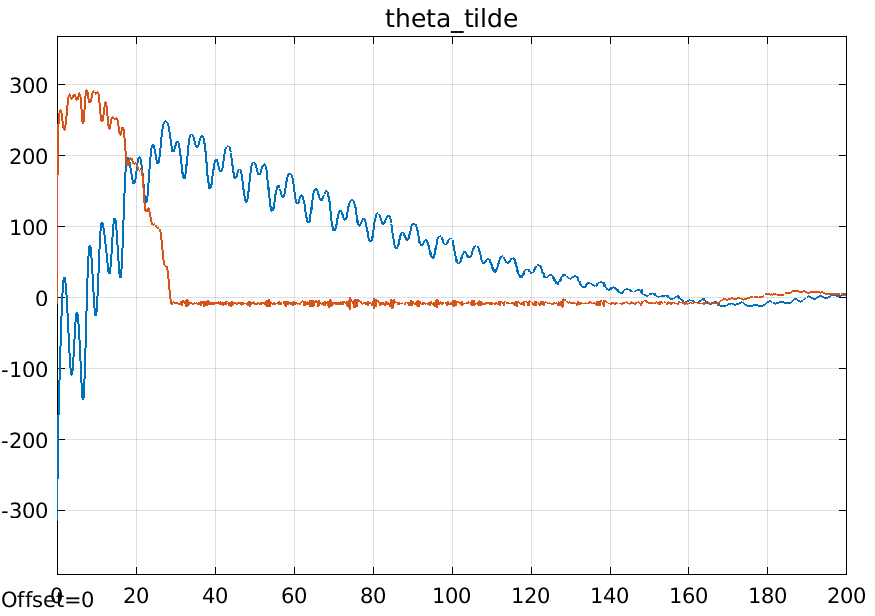
\includegraphics[width=0.59\textwidth]{3-2-1-theta}
			\caption{Вектор параметрических ошибок $\tilde{\theta}$ при $\gamma=1000$}
			\label{fig:3-2-1-theta}
		\end{figure}
		
		Теперь выберем $\gamma=200$. Полученные графики представлены на рисунках \ref{fig:3-2-2-x}-\ref{fig:3-2-2-theta}.
		
		\begin{figure}[H]
			\centering
			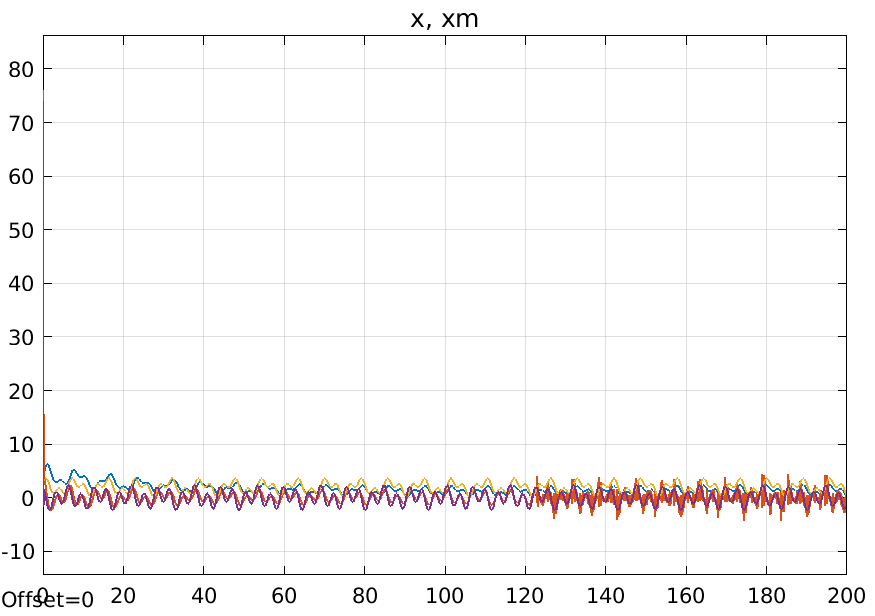
\includegraphics[width=0.59\textwidth]{3-2-2-x}
			\caption{Вектора состояния модели $x$ и эталонной модели $x_M$ при $\gamma=200$}
			\label{fig:3-2-2-x}
		\end{figure}
		
		\begin{figure}[H]
			\centering
			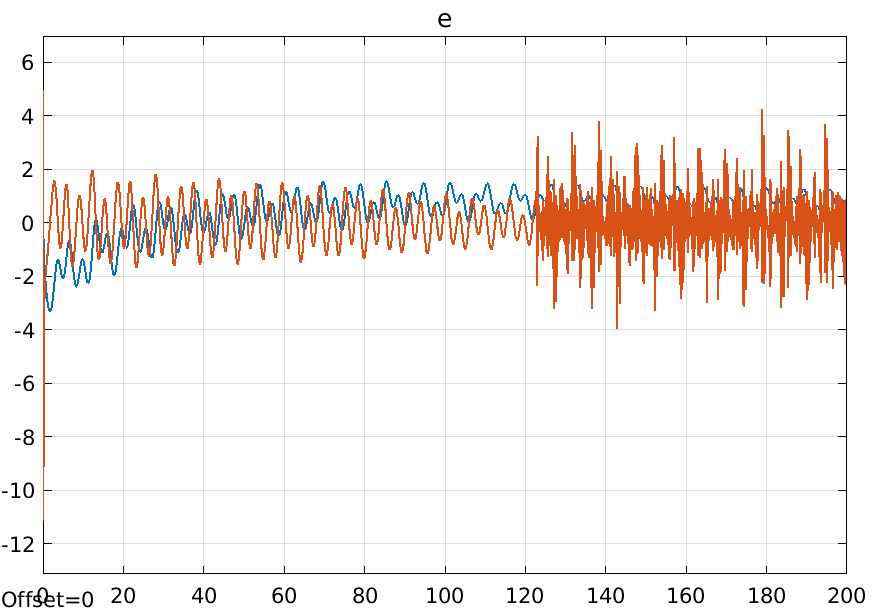
\includegraphics[width=0.59\textwidth]{3-2-2-e}
			\caption{Вектор ошибки управления $e$ при $\gamma=200$}
			\label{fig:3-2-2-e}
		\end{figure}
		
		\begin{figure}[H]
			\centering
			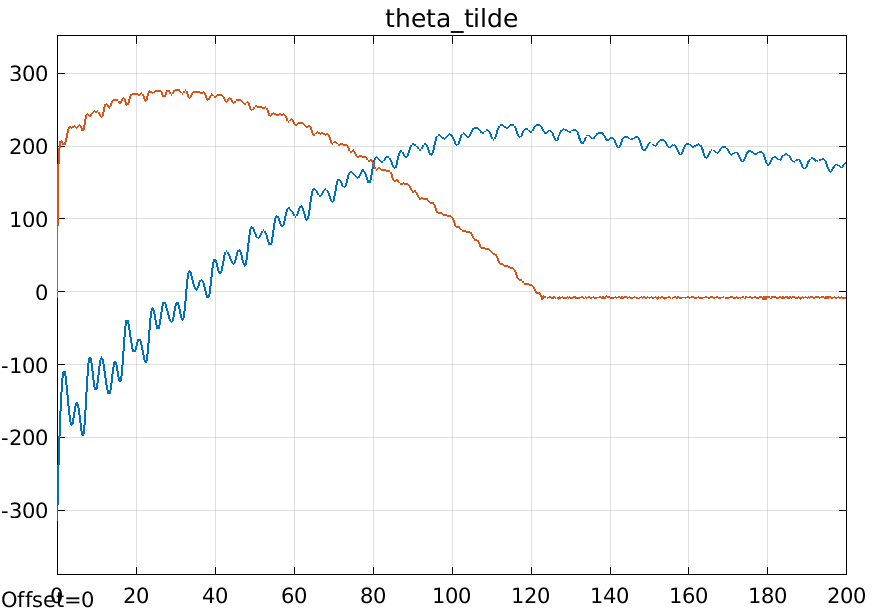
\includegraphics[width=0.59\textwidth]{3-2-2-theta}
			\caption{Вектор параметрических ошибок $\tilde{\theta}$ при $\gamma=200$}
			\label{fig:3-2-2-theta}
		\end{figure}
		
		Вернем $\gamma=100$ и проведем моделирование при $g(t)=1$. Полученные графики представлены на рисунках \ref{fig:3-3-x}-\ref{fig:3-3-theta}. 
		
		\begin{figure}[H]
			\centering
			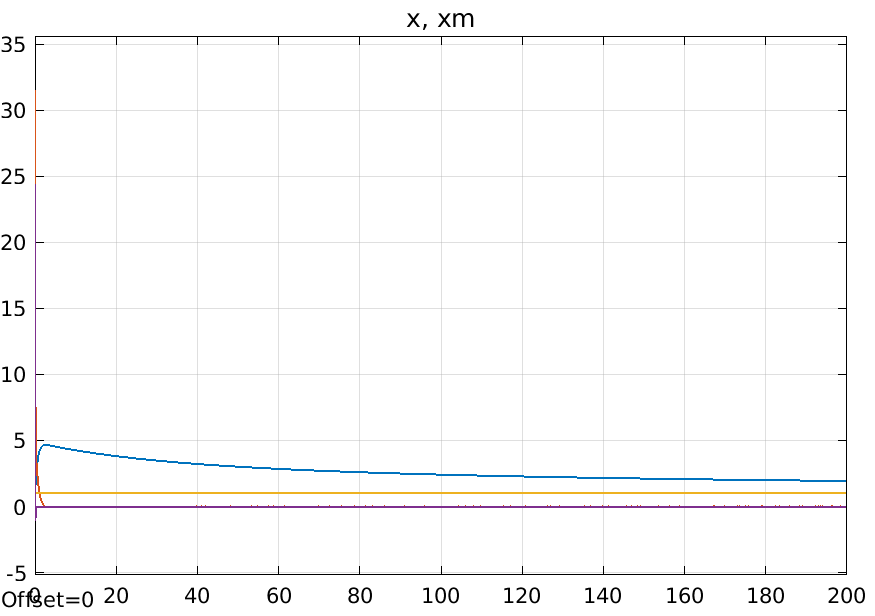
\includegraphics[width=0.59\textwidth]{3-3-x}
			\caption{Вектора состояния модели $x$ и эталонной модели $x_M$ при $g(t)=1$}
			\label{fig:3-3-x}
		\end{figure}
		
		\begin{figure}[H]
			\centering
			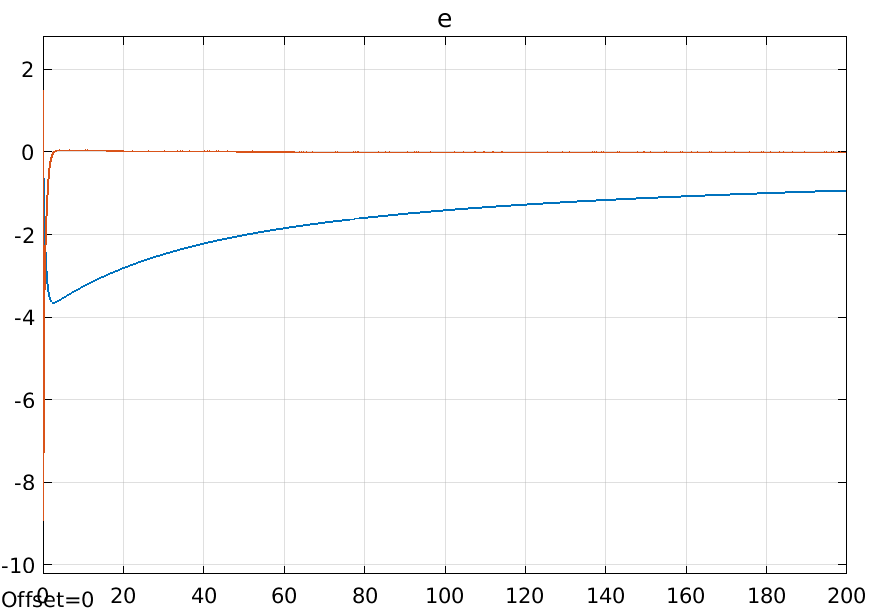
\includegraphics[width=0.59\textwidth]{3-3-e}
			\caption{Вектор ошибки управления $e$ при $g(t)=1$}
			\label{fig:3-3-e}
		\end{figure}
		
		\begin{figure}[H]
			\centering
			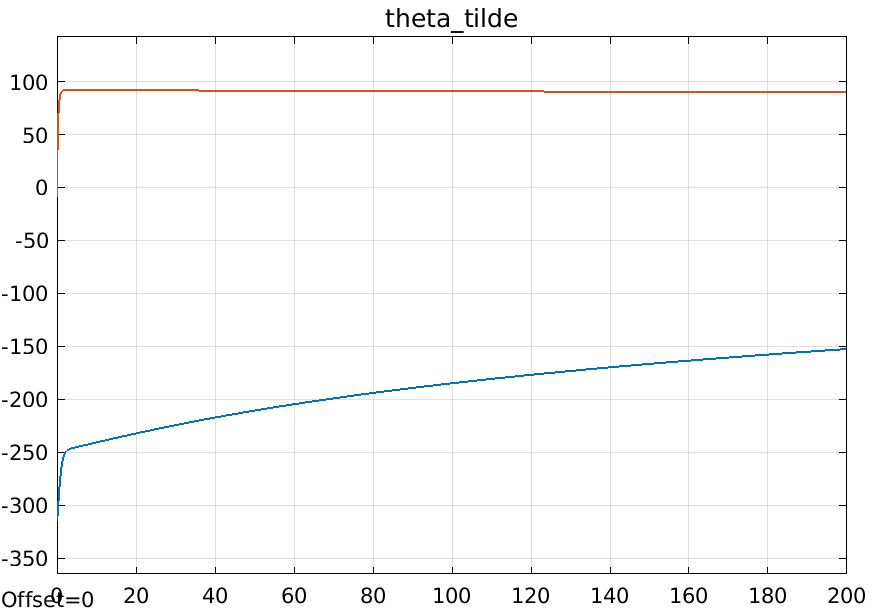
\includegraphics[width=0.59\textwidth]{3-3-theta}
			\caption{Вектор параметрических ошибок $\tilde{\theta}$ при $g(t)=1$}
			\label{fig:3-3-theta}
		\end{figure}
		
	\end{enumerate}
	
	\newpage
	
	\section*{Вывод}
	
	При моделировании адаптивной системы управления была представлена ограниченность всех сигналов в замкнутой системе даже при изменении параметров объекта управления.
	
	Также при любом $\gamma$ можно наблюдать асимптотическое стремление ошибки $e$ к нулю. При увеличении $\gamma$ увеличивается скорость сходимости параметрических ошибок $\tilde{\theta}$ к нулю.
	
	Также было показано, что для экспоненциального стремления вектора $\hat{\theta}$ к $\theta$ необходимо наличие не менее $(n+1)/2$ гармоник в сигнале $g(t)$.
	
	
\end{document}